\chapter{Methodology}
\todo[inline]{POS tagging; Dependency Parsing ; TM; TBL}

%\atrcomments{TBD!!!!!}



\section{Corpus}
\todo[inline]{EACL+ICON}
\subsection{Data Sets}


For our experiments, we use the Wall Street Journal (WSJ) section of the Penn Treebank \cite{marcus:kim:ea:94} and the GENIA Corpus (version 3.02) \cite{tateisi:tsujii:04}. Both corpora use the Penn Treebank POS tagset \cite{santorini:90} with minor differences.%, as described in section \ref{sec:q1}.

For the WSJ corpus, we extract the POS annotation from the syntactically annotated corpus. The GENIA Corpus comprises biomedical abstracts from Medline, and it is annotated on different linguistic levels, including POS tags, syntax, coreference, and events, among others. We use the POS tagged version. For WSJ, we use the standard data split for parsing:  using sections 02-21 as training data and section 22 as our test set. We reserve section 23 for future parsing expert experiments.


\section{Topic Modeling}

Probabilistic topic modeling is a class of algorithms which detects
the thematic structure in a large volume of documents. Topic modeling
is unsupervised, i.e., it does not require annotated
documents \cite{Blei:2012:PTM:2133806.2133826} but rather discovers similarity between documents. Latent Dirichlet
Allocation (LDA) is one of the topic modeling algorithms. It is a
generative probabilistic model that approximates the underlying hidden topical structure of a collection of texts based on the distribution of words in the documents \cite{Blei:2003:LDA:944919.944937}. I explain LDA in more detail below.

\paragraph*{LDA} 

Intuitively, Latent Dirichlet Allocation (LDA) is a method for discovering the hidden topics in a sentence. E.g., consider the following WSJ sentence. If we choose to model this in terms of LDA, we get the output shown in table~\ref{tab:2topicssent} and \ref{tab:10topicssent}.


``Though growers can't always keep the worm from the apple , they can protect themselves against the price vagaries of any one variety by diversifying -- into the recently imported Gala , a sweet New Zealand native ; the Esopus Spitzenburg , reportedly Thomas Jefferson's favorite apple ; disease-resistant kinds like the Liberty."
 
 % Please add the following required packages to  document preamble:
%\usepackage{multirow}
\begin{table*}[!htb]
\centering

\caption{2 topics distribution}
\begin{tabular}{cc}
%\multicolumn{2}{c}{2-topic probability distribution} 
\\ \hline
0 & 1 \\
95.90 & 4.10 \\ \hline
\end{tabular}
\label{tab:2topicssent}

\caption{10 topics distribution
%\\ 
}
\begin{tabular}{cccccccccc}
%\multicolumn{10}{c}{10-topic probability distribution} 
\\ \hline

0 & \multicolumn{1}{c}{1} & \multicolumn{1}{c}{2} & \multicolumn{1}{c}{3} & \multicolumn{1}{c}{4} & \multicolumn{1}{c}{5} & \multicolumn{1}{c}{6} & \multicolumn{1}{c}{7} & \multicolumn{1}{c}{8} & \multicolumn{1}{c}{9} \\
0.11 & 0.10 & 0.08 & 0.10 & 0.09 & 30.58 & 15.28 & 49.55 & 3.93 & 0.16 \\ \hline
\end{tabular}
\label{tab:10topicssent}

%\caption{2 \& 10-topic probability distribution for a WSJ corpus sentence: \\ }
%\label{tab:10t-probab}
\end{table*}

I.e., when we choose the number of topics as 2 \& 10, LDA creates a probabilistic distribution of topics in the sentence. This process of discovering topics in a document can be represented by a generative model. Figure~\ref{fig:ldaplate} shows the plate diagram for graphical model for LDA. Plate diagrams are standard for representing repeating entities in a graphical model for Bayesian inference. Each document($W$), i.e., a sentence in this case, is a mixture of topics. In other words, a sentence consists of a collection of words, i.e., $W = {w_1,w_2, ..., w_N}$. A corpus can be represented as a collection of $M$ sentences or documents, i.e., $C = {W_1, W_2, ..., W_M}$. For each sentence in a corpus, the generative steps for LDA can be given as below:
\begin{itemize}
    \item The number of words in a sentence i.e., $N$ is chosen from a Poisson distribution.
    $$N \sim Poisson(\lambda)$$
    \item The mixture of topic for a sentence is chosen according to the dirichlet distribution over a fixed set of topics.
    $$\theta \sim Dirichlet(\alpha)$$
    \item Each word ($w_i$) in sentence ($W$) can be generated as follows:
    \begin{itemize}
        \item Pick a topic according to the multinomial distribution sampled above.
        $$Z_n \sim Multinomial(\theta)$$
        \item Generate the word from the topic according to the multinomial distribution of topics. I.e., we choose a word from $p(w_n|Z_n, \beta)$, where $\beta$ represents word probabilities.
    \end{itemize}
    
    
\end{itemize}

The inference/parameter estimation step follows the generative step, which requires calculating the posterior distribution of the hidden variables given a sentence. 
\atrcomments{to be finished ........}




\begin{figure*}[t]
    \centering
    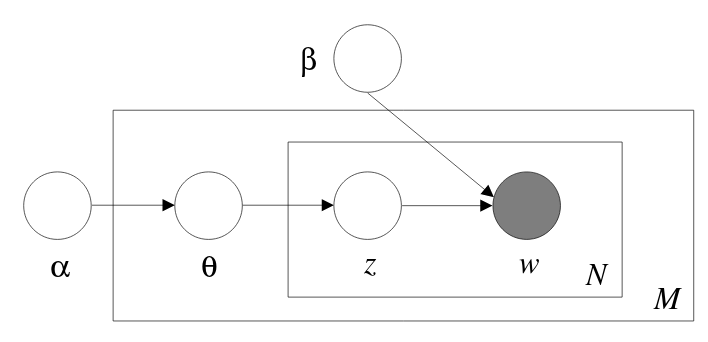
\includegraphics[width=\textwidth]{figures/LDA_plate_diagram.png}
 \caption{Graphical model for LDA~\citep{Blei:2003:LDA:944919.944937}}\label{fig:ldaplate}   
 \end{figure*}
 

\paragraph*{LDA toolkit}

There are several  open sourced toolkits available for LDA. We use the topic modeling toolkit MALLET \cite{McCallumMALLET}.  The
topic modeler in MALLET implements Latent Dirichlet Allocation (LDA), clustering
documents into a predefined number of topics. As a result, it provides
different types of information such as:

\begin{itemize}
	\item  Topic keys:  The highest ranked words per topic with their probabilities; 
	
	\item Document topics: The topic distribution for each document (i.e., the probability that a document belongs to a given topic); and 
	
	\item Topic state: This correlates all words and topics.
	
\end{itemize}

\section{POS Tagging}

\paragraph*{POS Tagging Toolkit}

For part of speech tagging, I use the TnT (Trigrams'n'Tags) tagger \cite{brants:00.2}. TnT is based on a second order Markov Model and has an elaborate model for guessing the POS tags for unknown words. I use TnT mainly because of its speed and because it allows the manual inspection of the trained models (emission and transition frequencies).

\section{Dependency Parsing}

The process of automatically analyzing dependency structures to an input sentence is referred to as dependency parsing. A dependency tree needs to satisfy the following properties~\cite{kubler2009dependency}:
\begin{itemize}
\item A dependency tree needs to have an artificial root which specifies that there there must not exist an arc which comes into the root from another node(word).
\item A dependency tree must satisfy the spanning property for all the words in a sentence.
\item A dependency tree must be connected i.e., if we ignore the directed edges then every word in a sentence must be connected.
\item Every word in the dependency tree must have one head only.
\item A dependency tree must be acyclic, i.e., should not contain cycle.
\item Number of arcs in the dependency tree must be one less than the number of words, i.e., $$|E| = |W| - 1$$ for a dependency tree $G = (W,E)$ where E is number of arcs and W is number of words.
\end{itemize}

There are two different kinds of dependency structures based on which, dependency trees can be categorized into two types. Figure~\ref{fig:proj-non-proj} shows an example illustrating the difference between projective (right) and non-projective (left) trees.  

\begin{figure*}[!htb]
    \centering
    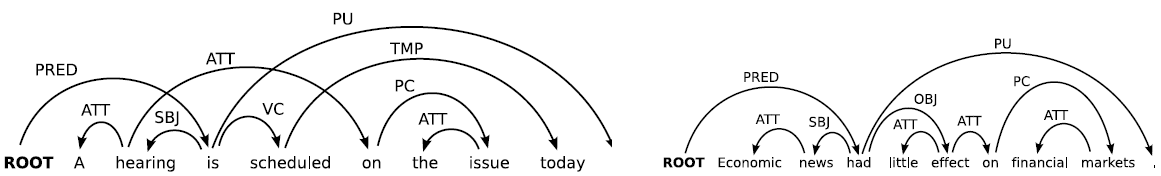
\includegraphics[scale = 0.45]{proj-non-proj.png}
    \centering
    \caption{Projective and Non-projective dependency trees~\cite{kubler2009dependency}}
    \label{fig:proj-non-proj}
\end{figure*}

\begin{itemize}
    \item Projective dependency trees - For these dependency trees, the dependencies do not cross each other. Usually, the sentences in English are projective.
    \item Non-projective dependency trees - For these type, the dependency branches can cross each other. This is more prevalent in the languages with free word order like German.
    
\end{itemize}


There are two major approaches for this problems - data-driven and grammar-based. The grammar-based approaches make use of a formal grammar and the problem in this case is defined as - whether the input sentence belongs to the language defined by this formal grammar. In contrast to grammar-based approaches, data-driven approaches utilize machine learning approaches on annotated data from a corpus to parse a given input sentence. Since data-driven approaches rely on machine learning approaches, we will only discuss these methods in the rest of the report.

\begin{itemize}
    \item{Transition-based - }{In a transition-based approach are based on the notion of transition system which is a finite state automaton. An FSA consists of states, transitions, mapping states and input symbols and transitions from initial to final states. The state transition happens on an input to a state. In case of transition based parsing, each of the states represent steps for deriving a dependency tree. These approaches make use of a stack-based technique for parsing. Transition based systems are mostly stack-based. Initially, the stack contains the artificial root and the buffer is empty. There are three kinds of transitions - shift, left and right. This is a bottom-up approach, i.e., for an arc to be constructed between two nodes, it is imperative that the dependent node has already a dependency tree constructed. This approach is also known as arc-standard. There is another approach called arc-eager where the terminal configuration is guided by the state of the buffer. If it is empty the arc-eager system terminates. In addition to the transitions in the arc-standard system, there is an additional transition called reduce. This is a top-down parsing approach as the arcs are added as and when found~ \cite{kubler2009dependency}.
    }
    \item{Graph-based - }{Graph-based approaches rely on the algorithms for directed graphs like finding the maximum spanning trees. There is a scoring function which evaluates how correctly a particular tree analyzes a sentence~\cite{kubler2009dependency}. }
\end{itemize}
 
Various machine learning techniques have been implemented in different stages of parsing. In general, machine learning algorithms are used to compute scores in case of graph-based algorithms while for transition-based systems, it is used as an oracle. Supervised learning methods have proven useful while most recently, semi-supervised and unsupervised methods have shown promise. The goal is to reduce the time taken in parsing while not compromising the quality of the parse. 
The parsing problems by using these approaches are discussed in further details in the subsequent sections. We have further sub-categorized problems by whether they work for projective or non-projective sentence structures. Usually, the problem with projective sentences are a subclass of that of the non-projective sentences. The pseudo-projective approaches are also listed under the non-projective approaches. Neural network approaches are categorized in a separate section for ease of readability.

%\subsection{Discriminative Models}
\subsection{Transition based approaches}

Broadly, there are two main approaches to transition based parsing. 

\begin{itemize}
\item Greedy classifier based - The transition-based approach has a set of transitions between the states (or configuration). However, to categorize this as a parsing problem, we need to score these transitions and estimate the highest scoring transition by using a model. A classifier can be used as this model which maps configurations to the most optimal transition. The optimal transition can be determined in a greedy way, where the final optimal transition is determined by selecting the optimal transitions locally. A representation of the scoring is as below:
\begin{equation*}
Score(C, T) = \sum_{i = 1}^{N} f_i(C,T).w_i
\end{equation*}
where C = configuration, T = transition
Many machine learning techniques are used to learn the weights such as SVMs, perceptrons, etc.(more recently, neural networks)

\item Beam search and structure learning - The beam search and structure learning has a similar strategy, however, in this case, instead of a greedy search, beam search is applied. Thus instead of 1 optimal transition, $n$ number of possible optimal solutions are considered at each step where $n$ is the beam size. The second part is similar to greedy classifier method, except that it has been seen (as we will see later in this chapter) that structured learning approaches tend to have better results.
\end{itemize}

We discuss the existing methods for transition based learning from the point of view of projectivity. Since our objective is to highlight the machine learning approaches, we will look at it from the perspective of the machine learning techniques used.

\subsubsection{Projective}

Probabilistic approaches to parsing initially showed promising results in dependency parsing as compared to rule-based techniques. 
%A simple bigram probabilities estimation technique was used to estimate the probability of dependencies between pair of words for the Wall Street Journal corpora~\cite{Collins:1996:NSP:981863.981888}. 
%Decision trees~\cite{haruno1999using} and Maximum Entropy models~\cite{Charniak:2000:MP:974305.974323} were also implemented for dependency structure analysis. However, these approaches did not address the feature selection or in other words, how selecting good features could be a key in improving the results in dependency structure analysis. So, 
Previous work in syntactic parsing (constituency parsing, in most cases) did not address the feature selection or in other words, how selecting good features could be a key in improving the results in dependency structure analysis.
So, Kudo and Matsumoto\cite{Kudo:2000:JDS:1117794.1117797} applied Support Vector Machines (SVMs) for analysis of dependency structure in Japanese. They assume that the dependency structure holds the following constraints.
\begin{itemize}[leftmargin=*]
\itemsep-0.5em
    \item Each item depends on exactly one item appearing to the right.
    \item The dependencies are projective.
\end{itemize}
Since, the problem of statistical dependency analysis deals with finding the best dependency structure($D_{best}$) given a sequence of chunks of a sentence ($B$) (chunks are specific to Japanese dependency structure and are defined as relation between phrasal units), it can be formulated as follows:
\begin{equation*}
    D_{best} = \arg\max_{D} P(D|B)
\end{equation*}
Considering the dependent probabilities are independent of each other, $P(D|B)$ can be written as:

\begin{equation}
P(D|B) = \prod_{i=1}^{m-1}P(Dep(i)=j|f_{ij}) 
$ where, $ 
f_{ij} = {f_1,...,f_n} \in R^n 
\end{equation} \\
$P(Dep(i)=j|f_{ij})$ denotes the probability that the chunk i depends on the chunk j given an n-dimensional linguistically-motivated feature set. 
To find $D_{best}$, the authors have used the backward beam search technique for statistical dependency analysis of Japanese sentence by~\cite{Sekine:2000:BBS:992730.992755} which processes a sentence backwards.

The feature set consists of static features such as, head words and their parts-of-speech, particles and inflection forms of the words appearing at the end of chunks, distance between two chunks, existence of punctuation marks. In order to handle long sentences, dynamic features are included which resolves syntactic ambiguity at the time of parsing. These are mainly ``form of functional words or inflection that modifies the right chunk". The authors report a better accuracy compared to the previous work on the same corpus.

A similar discriminative model for dependency analysis on Wall Street Journal section (02-21 for training and 23 for test) of the Penn Treebank~\cite{Marcus:1994:PTA:1075812.1075835} using SVMs by Yamada and Matsumoto\cite{yamada2003statistical}.  They apply a deterministic bottom-up parsing algorithm which comprises of three actions - \textit{Shift}, \textit{Left} and \textit{Right}. The parsing algorithm undergoes a two-step procedure to parse an input sentence considering words from left to right. The first procedure involves assessing the appropriate action (\textit{Shift} or  \textit{Left} or \textit{Right}) from the contextual information provided by the surrounding words. Then, the parser builds the dependency tree by executing these actions determined in the previous step. During the training phase, each sentence is parsed using this algorithm. The contextual features with the right parsing action serves as an example for the SVM. Thus the estimation phase is a multiclass classification problem comprising of three binary classifiers for each action in a pairwise fashion:
\begin{itemize}[nolistsep,leftmargin=*]
%\itemsep-.75em
\item Left vs. Right
\item Left vs. Shift
\item Right vs. Shift
\end{itemize}
The decision on the action that needs to be implemented at any stage is determined by the cumulative votes from each of these SVMs. 
The features are as follows:
\begin{itemize}[nolistsep,leftmargin=*]
%\itemsep-.25em
\item word
\item Part of Speech (POS) tags
\item child word modifying the parent node on the right hand side
\item child word modifying the parent node on the left hand side
\item POS tag of the child node modifying the parent node on the right hand side
\item POS tag of the child node modifying the parent node on the left hand side
\end{itemize}
Each feature is defined as a triplet consisting of the position from target node, feature type and the feature value. The accuracy of this parser is not at par with the contemporary phrase structure parsers owing to the fact that the phrase structures are not utilized in this parser. Malt parser (discussed in the non-projective section) addressed the problems faced by this parser viz., requirement to iterate for long sentences.

Cheng~\etal~\cite{cheng2005chinese} applied a similar approach using SVMs to determine if a dependency relation exists for any two pair of words based on  Chinese Treebank. The parsing method is based on Nivre and Scholz's~\cite{Nivre:2004:DDP:1220355.1220365} bottom-up deterministic algorithm which parses a sentence in linear time. The basic difference is in the machine learning algorithm used for these two papers. While Nivre and Scholz used memory based learners ($5$-nearest neighbors (IB 1) from TiMBL~\cite{daelemans2004timbl}). This algorithm is also stack-based, where the analyzer states are represented as a triple $\langle S, I, A \rangle$ where $S$ contains the words which are being considered, $I$ contains the words which are to be processed and $A$ is a list of dependency relation. 
It is also important to point out the differences between Yamada and Matsumoto's approach to that of Nivre's since both are based on English text and use a deterministic parsing algorithm. The primary difference would be the choice of classifiers, SVMs vs. MBL. Yamada and Matsumoto's parser requires multiple passes but Nivre's take one pass which makes Yamada's algorithm's worst case time complexity to be quadratic as compared Nivre's algorithm's linear time.
The data-driven dependency parsing was further used for parsing Swedish~\cite{nivrej.2004}, Bulgarian~\cite{marinov2005data} and Turkish~\cite{eryiugit2008dependency} treebanks with improvement over baseline.

At any stage, there are four possible operations for a given configuration - right, left, reduce \& shift. Right \& left operations add dependencies based on whether the top word in $I$ depends on the top word in $S$ or in the other direction respectively. For reduce, if the top element of $S$ has no dependents, it is removed. For shift, the analyzer checks whether there is any possible dependency relation between the top elements of $S$ and $I$. If it does not find one and the conditions for reduce are not met as well, then the top element of $I$ is pushed into $S$.

Since the two methods (Cheng vs. Nivre) use different machine learners, the feature set is different. Nivre and Scholz considered the top word of the stack, the next input token, left and right dependent of the top element in the stack, left dependent of the next input token, the possible tokens from next configurations which are connected through a dependency arc. For the tokens in consideration, the lemma and part of speech tags are considered, while for the ``lookahead" tokens, they have only considered the part of speech tags. For Cheng's work, each node comprises of the word, POS tags and information of its children. They also take context features, such the preceding and succeeding nodes and its children into consideration. These are treated as local features. The global features are used for the long distance dependencies. If the local features arrive at a decision which is shift/reduce, the analyzer uses SVMs to determine the correct operation using global features. They have also proposed a two-step process for finding the root words using SVMs. They have reported an increase in accuracy by employing the global features and the root word finder. 

This method was further extended to account for multiword units (MWUs) such as multiword names, function words by Nivre and Nilsson~\cite{nivre2004multiword}. Particularly, to examine whether multiword units help in improving the parser results and if so, at which point should this be implemented. They experimented on the lexicalized and non-lexicalized versions of the parser based on memory-based learning. They show a significant improvement over the baselines for the syntactic structures in addition to the MWUs.

In order to analyze whether there is a ``better" machine learning algorithm for parsing, Hall~\etal~\cite{Hall:2006:DCD:1273073.1273114} presented a comparison between SVMs and memory based learning classifiers in deterministic dependency parsing for English, Chinese and Swedish using a variety of features. They show that the accuracy achieved by these classifier based models are almost at par with more complex parsing models. For their experiments, SVMs outperform the memory based learners but with a tradeoff in training times.

\paragraph{Pseudo projective approaches}

English sentences are generally projective, i.e., the edges of the dependency trees do not cross each other in a sentence. However, in the languages with a flexible word order like German, Czech and Dutch, the sentences tend to be non-projective with crossing dependencies. To solve, this problem, Nivre and Nilsson~\cite{nivre2005pseudo} devised a ``pseudo projective" method for parsing and reported an improvement over the state-of-the-art non-projective parsing results for Prague Dependency Treebank~\cite{bohmova2003prague,hajic1998building} by using a combination of data-driven deterministic dependency parsing (memory-based) with a graph transformation technique called lifting. Typically, a non projective dependency graph can be converted to a projective one by replacing the non-projective arc with a projective one. The authors have implemented a transformation involving a minimal number of lifts. Thus, at the first step, the dependency trees are projectivized by applying the minimal lift transformation technique. In the second step, they have implemented an inverse transformation based on the breadth-first search algorithm using three encoding schemes. As a part of the experiments, memory based dependency parsers are used and the projectivized trees are used for training. The output is transformed using the inverse transformation and compared to the gold standard test set.

\subsubsection{Non-projective}

While the parsing techniques for English have proven to be efficient enough, parsing non-projective tree structures can prove to be challenging. A lot of techniques, as we will see later for the generative models as well, work for non-projective sentences with some modification on the projective counterparts. 
          
This problem has been addressed by Nivre~\etal\cite{nivre2006maltparser,nivre2007maltparser}, who introduced MaltParser, which they describe as ``data-driven parser-generator for dependency parsing". The parser requires a treebank and not a grammar unlike contemporary parser-generators. The parsing comprises of - building dependency graphs by deterministic parsing algorithms as shown by Yamada and Matsumoto and Nivre, estimating the next action of the parser by building a history-based feature model and finally mapping the history to parser action using discriminative machine learning algorithms (as demonstrated in Yamada and Matsumoto's and Nivre's work) such as memory based learning, SVMs. MaltParser specifies a fized set of data structures and typically any parsing algorithm which follows this architecture would work in the framework. It supports Nivre's~\cite{nivre2003efficient}[An efficient algorithm for projective dependency parsing] and Covington's~\cite{covington2001fundamental} algorithms which uses three approaches - Brute-force search, Exhaustive left-to-right search and enforcing uniqueness. The feature models consists of word, lemma, part of speech tags, dependency type described in terms of the provided data structures. The evaluations provided by Nivre~\etal for MaltParser is for Swedish, English, Czech, Danish and Bulgarian based on memory based learning.

It is clear that, parsing accuracy and time is an issue for non-projective parsing, which caused largely due to the way non-projective dependencies are handled. Also, it has been argued that, even for the free word order languages, the dependency structures tend to be either projective or ``very nearly projective". This leads to the discussion of finding the appropriate ``degrees of non-projectivity"~\cite{nivre2006constraints}, which can be stated as finding a balance such that a small amount of non-projectivity might improve the parsing accuracy and time over strict projectivity and it is also more efficient than considering non-projectivity in abundance. Nivre~\cite{nivre2007incremental} investigated this appropriate degree of non-projectivity by using Covington's parsing algorithm with history based SVM classifier to  predict the next parser action. The results indicate that the languages exhibiting extensive non-projectiveness, the parser accuracy can be boosted if the non-projective dependencies are derived. However, on the other hand, parsing times can be improved by curbing the non-projectivity with a small decrease in parsing accuracy. 

Although SVMs work well in case of parsing, it can be expensive in terms of training and memory requirements. A better workaround for this can be, to use multi layer perceptrons as the classifier~\cite{attardi2009accurate} as perceptrons are faster and require less memory.  



%\cite{bohnet2010very}

%A Transition-Based System for Joint Part-of-Speech Tagging and Labeled Non-Projective Dependency Parsing

%Getting the Most out of Transition-based Dependency Parsing

%Transition-based Dependency Parsing with Rich Non-local Features


%\subsection{Generative Models}

\subsection{Graph based approaches}

The most basic model for graph based parsing is the arc-factored model. An arc is an edge in the dependency tree. This is also commonly referred to as the first order model since the score is computed based on the scores of each arc. This is an exact inference. However, research has indicated that better parsing accuracy can be achi  eved when we considered bigger subgraphs i.e., set of 2 or 3 arcs in dependency tree. These models are referred to as second and third order models respectively but it increases the parsing complexity i.e., for learning and parsing. These are approximate inferences. In the subsequent sections, we have divided graph-based models in terms of projectivity and non-projectivity. 



\paragraph*{Eisner's Algorithm}
Quite a lot of work has been done using generative models to improve the results of dependency parsing. To address the ``lexical blindspot" of context-free grammars (CFGs), Eisner~\cite{eisner1996three} proposed three different probabilistic approaches to describe the basic structure of a sentence and apply it to a dependency framework for improving the resulting parses. This is a constituent CKY based algorithm for dependency parsing which uses words as node labels. This has been used for parsing projective dependencies The probabilistic models are as follows:

\begin{figure*}[!htb]
    \centering
    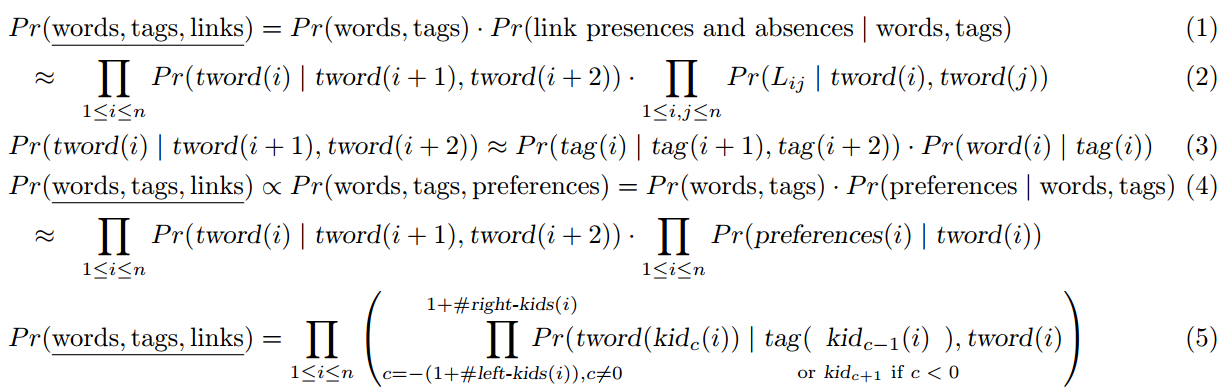
\includegraphics[scale = 0.45]{Eisner.png}
    \centering
    \caption{Three probabilistic models in Eisner's work}
    \label{fig:eisnerexpressions}
\end{figure*}

\begin{itemize}

\item Bigram lexical affinities [expressions 1-3 in Fig.~\ref{fig:eisnerexpressions}]

The first step is to generate tags by a Markov process given the previous two tags. Next, a word is chosen, given each tag. To account for the dependencies, there is a third step in this process which considers pairs of words and makes a random decision whether to link the two based on whether the probability of the words being linked together is ``lexically sensitive". I.e., both the tag and word are considered for any pair of words. This model also accounts for the inter-dependencies between the children of a word.

\item Selectional preferences [expressions 4 in Fig.~\ref{fig:eisnerexpressions}]

A sequence consisting of word and its tags are generated by a Markov process and then for each word, a parent is described. Hence the ``selectional preference"\footnote{referred to as disjunct, in the paper} for each word is being considered in this case. Then, each of the words are independently ``sense tagged" based on its selectional preference.

\item Recursive generation [expressions 5 in Fig.~\ref{fig:eisnerexpressions}]

This is a generative model as opposed to the two previously described comprehensive models. Every time a word is added, two separate Markov sequence of tag/word pairs are generated to serve as its left and right children. This process continues recursively for each child which is generated.

\end{itemize}

A probabilistic algorithm which is similar to CKY is proposed as the parsing algorithm. CKY considers substrings of increasing length for parsing and thus each such substring is represented as lexical trees. But, in this case, instead of considering substring as trees, the parser considers these as spans. These approaches when tested on the WSJ corpus indicate that the recursive generation model performs better as compared to the other two. The parsing algorithm has a $O(n^3)$ complexity. 

Training these models is particularly easy as it constitutes mainly of estimating probabilities by counting the events related to parsing in the training set. However, this advantage is sometime nullified due to the poor decisions in the independence assumptions. This is where the discriminative models tend to perform better. However, these especially Maximum Entropy Markov Models based parsers~\cite{ratnaparkhi1999learning} tend to run into the label bias problem (\atrcomments{?}) because it does not take the parsing decisions based on an observation which might be seen later in the sequence. Parsing the training corpus repeatedly can solve this problem to some extent. However, it is really expensive - $O(n^5)$ as opposed to $O(n^3)$ for generative models. Hence, to strike a balance and utilize reduced parsing complexity of generative models like Eisner's, McDonald~\etal~\cite{McDonald:2005:OLT:1219840.1219852} described a method of training dependency parsers for English and Czech using margin-sensitive online training algorithms~\cite{crammer2003ultraconservative,shalev2003online}. The authors mention that this method can be translated for non-projective cases (where it may appear in Czech, for instance) as well. Since the reported results are for projective cases only, we have listed it so.



\paragraph*{Chu-Liu-Edmonds Algorithm}

Chu-Liu-Edmonds algorithm\cite{chu1965shortest,edmonds1967optimum} often serves as a basis for non-projective parsing approach which determines the maximum spanning tree (MST) of a graph in a greedy and recursive way. We will informally explain the intuition behind the algorithm as follows:
\begin{itemize}[label={--}]
\item{Motivation: } All the nodes in a graph need to be in arborescence. I.e., there should be exactly one directed path between two nodes in the graph.
\item An incoming edge is selected for a node in a greedy way.
\item The highest scoring incoming edge is stored for every non-root node.
\item If a cycle is formed, a decision has to be made to remove one of the nodes to resolve the cycle. 
\item There are two stages - contract and expand. 
\item Following steps are followed for contract phase:
\begin{itemize}[label=$\diamond$]
\item At first, the nodes in a cycle are contracted to form a new node/vertex.
\item All the incoming edges to the nodes in the cycle are now redirected to the new node.
\item Similarly, the outgoing edges have the new vertex as its starting vertex.
\item  The incoming and outgoing edge weights for this new ``contracted" vertex are recalculated.
\item This process is repeated recursively until every non-root vertex contains exactly one incoming node and there are no cycles.  
\end{itemize}
\item The MST formed on this contracted graph can be shown to be equivalent to MST for the original graph. \cite{georgiadis2003arborescence}
\item Thus the algorithm is recursively implemented on the new graph to find the MST.
\end{itemize}


\paragraph{Non-projective approaches}
While the graph transformation techniques yielded good results with a cubic complexity, the parsing complexity was reduced by McDonald~\etal~\cite{McDonald:2005:NDP:1220575.1220641} who proposed a dependency framework for both projective and non-projective dependency parsing by formalizing the problem as searching for maximum spanning tree (MST). They have used a similar approach as Hirakawa's~\cite{hirakawa2001semantic} spanning tree search for dependency parsing. However, the worst case performance is exponential in this case as branch and bound algorithm is used. They used Eisner's spanning trees approach for projective and Chu-Liu-Edmonds algorithm~\cite{chu1965shortest,edmonds1967optimum} for non-projective dependency trees. At first, an edge-based factorization is applied to the projective languages with Eisner's parsing algorithm and Chu-Liu-Edmonds maximum spanning tree algorithm for non-projective languages. The edge factorization for an edge is done by computing a dot-product between a high dimensional feature representation of the edge in consideration and a weight vector. The score of a dependency tree is then a sum of the scores of all edges in the tree. The weight is updated by using the online learning algorithm implemented in McDonald~\etal~\cite{McDonald:2005:OLT:1219840.1219852}. Their results show significant improvement in accuracy even with a small amount of non-projective sentences. They also reported improved parsing times - $O(n^2)$ as compared to $O(n^3)$ - in favor of the Chu-Liu-Edmonds algorithm as opposed to Eisner's. Their parser performs well even when compared to state-of-the-art\atrcomments{?} lexicalized phrase structure parsers such as 
Collins~\etal~\cite{collins1999statistical} and Zeman~\cite{zeman2004parsing}, whose parsing complexity is $O(n^5)$. This framework was further account for higher-order feature representation and acyclic dependencies, i.e., multiple heads for each word~\cite{mcdonald2006online} by using approximate inferencing of the online learning algorithms. The defined approximation is to start with a reasonably good baseline structure and then continue making transformations until the structure converges. 

In order to devise more effective ways of solving multilingual parsing problems, McDonald~\etal~\cite{McDonald:2006:MDA:1596276.1596317} proposed a two-stage multilingual parser and evaluated it on the 13 language treebanks provided in different CoNLL shared tasks~\cite{Buchholz:2006:CST:1596276.1596305}. The first stage in this model is to create an unlabeled parse for an input sentence. They extend the existing models by McDonald \& Pereira~\cite{mcdonald2006online}, adding morphological features (where available) for each token. The morphological features (includes features for parent and its dependent and also various conjunctions of features from each of sets. The second stage is label classification which takes the output parse from stage 1 and assigns each edge with a label with the highest score. A first order Markov factorization has been used. Each factor is defined as the score of labeling adjacent edges. As defined in the earlier work by McDonald~\etal, the score function is defined as the dot product between the high dimensional feature representation and a weight vector. The most likely sequence of labels is then  ascertained by applying Viterbi's algorithm.


%paper= Online Large-Margin Training of Dependency Parsers

\paragraph{Higher order models}

As explained before, first order model is one in which the dependency tree os split into head and modifier dependencies. Second order models look into the adjacent dependencies in addition to these primary dependencies. McDonald \& Pereira~\cite{mcdonald2006online} experimented with second order graph models. Carreras~\cite{carreras2007experiments} extended this to experiment with other types of second-order relations. In particular, they look into PP-attachment which requires looking into grand parent relations. The training is done with averaged perceptron on Eisner's(1996) algorithm. Although it reported one of the best reported labeled attachment scores for some languages, this model suffers in terms of time and memory utilization. Bohnet~\cite{bohnet2010very} used this parser as a basis for their work on parallelizing the feature extraction and parsing algorithm by using passive-aggressive perceptron algorithm~\cite{crammer2006online} as Hash Kernel. The concepts from this model can be extended to the transition based parsers as well. Bohnet reported a 3.5 times increase in speed over the baseline MST parser using a single core CPU and it also requires a lot less memory than the contemporary parsers by using Hash Kernel. The speed increases further by using parallel algorithms and it can be further reduced at the cost of accuracy.


\subsection{Combining transition-based and graph-based models}


With the diverse amount of work on dependency parsers there has been work based on combining components from generative models with that of the discriminative approaches.

Graph-based and transition-based parsers have reported good accuracies for different criteria. Thus, a combination of both promises better results than individual. This premise was explored by Zhang \& Clark~\cite{zhang2008tale} for projective dependency parsing. They considered Malt and MST for transition and graph-based respectively. Their basis was to use of beam search framework. They have used perceptron for training and beam search for decoding. They tested the combined parser on English and Chinese with comparable results with that of the best parsers for both models.



CoNLL-X Shared Task on Multilingual Dependency Parsing~\cite{Buchholz:2006:CST:1596276.1596305} constituted multilingual parsing using a single dependency parser which can learn from treebank data. Nivre~\etal~\cite{Nivre:2006:LPD:1596276.1596318} used MaltParser to solve this problem for Swedish and Turkish. For mapping parser actions to history, they used SVMs and used graph transformations described by Nivre and Nilsson~\cite{nivre2005pseudo} to restore the non-projective structures.

\subsection{Unsupervised and semi-supervised approaches}


%From Baby Steps to Leapfrog: How “Less is More” in Unsupervised Dependency Parsing
%Unsupervised Induction of Tree Substitution Grammars for Dependency Parsing
%Viterbi Training Improves Unsupervised Dependency Parsing
%Punctuation: Making a Point in Unsupervised Dependency Parsing

%Simple Semi-supervised Dependency Parsing Terry Koo, Xavier Carreras, and Michael Collins

Some unsupervised and semi-supervised technieuqes have also been suggested to improve parser accuracy and addressing the concerns about portability of the system to other parsing frameworks. Blunsom \& Cohn~\cite{blunsom2010unsupervised} reported higher attachment scores by focusing on dependency grammar induction using tree substitution grammar because of its ability to learn large chunks of dependency tree. They devised a hierarchical non-parametric prior due to its bias towards simple productions. Spitkovsky~\etal~
~\cite{spitkovsky2010viterbi}, on the other hand, argued that Viterbi actually is better suited for the problem of grammar induction. They tested their approach on Brown corpus. However, there is no direct comparison with Blunsom's approach.

\subsection{Neural Network based approaches}

Although transition-based dependency parsers work reasonably well, but these parser tend to suffer due to poor estimation of feature weights, the incompleteness of manual feature templates and the time complexity for extraction of these features. The problem with sparse indicator features can be mitigated by using dense word embeddings as indicated in some of the recent works, such as for POS tagging~\cite{collobert2011natural}. Chen and Manning~\cite{chen2014fast} use a neural network based classifier for making the parsing decisions in a transition based dependency parser~\cite{Nivre:2004:DDP:1220355.1220365}. The architecture of the neural network based parser is given shown in figure~\ref{fig:NNchenmanning}. It contains exactly one hidden layer with a cubic  activation function ($g(x) = x^3$).

\begin{figure*}[!htb]
    \centering
    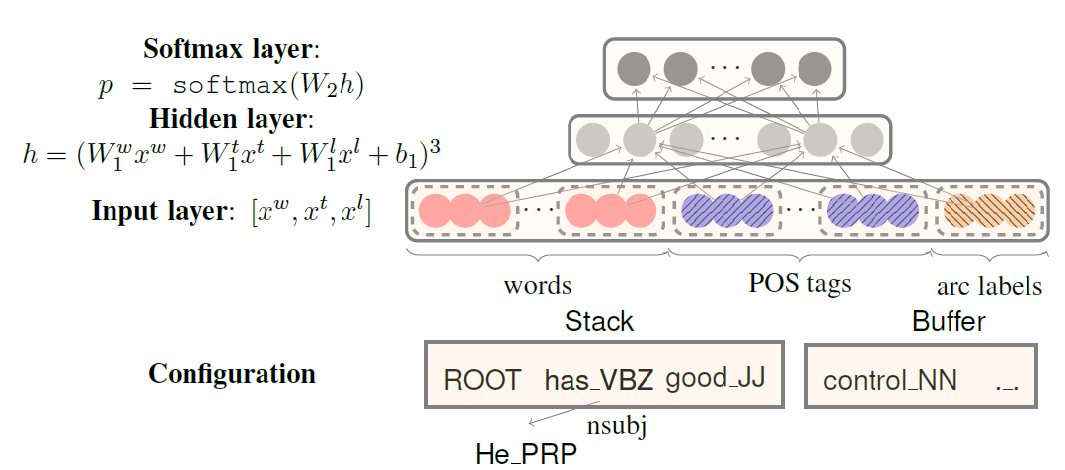
\includegraphics[scale = 0.5]{NNchenmanning.png}
    \centering
    \caption{Neural Network architecture}
    \label{fig:NNchenmanning}
\end{figure*}

A greedy decoding is performed for parsing. At every step, word, its POS and label embeddings are extracted from the current configuration and like all the transition based parsers, the transition with the highest score is selected. This work is shown for the projective case only. For the selected sentences in PTB and CTB, this parser works better than MaltParser and MST in terms of parsing time and accuracy. 
\cite{weiss2015structured} followed a similar approach but instead of one hidden layer, they added two which slightly improved the parser accuracy. Their work differs from Chen and Manning's by the use of semi-supervised structured learning which is implemented for the training. To learn the final layer of the model, they make use of structured perceptron. They also introduce unlabeled data by using word embeddings. This work was further extended for multilingual cases~\cite{alberti2015improved}. The difference is in the use of set or bag of features which are embedded into the same embedding space. 
Chen and Manning's neural network architecture for parsing was further modified by 
\cite{zhou2015neural} using beam search for the decoding step and contrastive learning to maximize the sentence-level log likeliood. They reported 1.8\% increase in accuracy over Chen and Manning's greedy neural parser.

A graph-based neural network parser was proposed by Pei~\etal~\cite{pei2015effective} which made use of a $tanh-cubic$ activation function instead of Chen and Manning cubic activation function. The parser outperformed the baseline graph-based parsers. However, it is not clear if this parser outperforms the other neural network based parsers. Neural network parsers for multilingual settings are implemented by using convolutional neural networks by Zhang~\etal~\cite{zhang2016probabilistic} by using the basic architecture of Pei~\etal.


\section{Domain Adaptation}